\documentclass[
	ngerman,
	toc=listof, % Abbildungsverzeichnis sowie Tabellenverzeichnis in das Inhaltsverzeichnis aufnehmen
	toc=bibliography, % Literaturverzeichnis in das Inhaltsverzeichnis aufnehmen
	footnotes=multiple, % Trennen von direkt aufeinander folgenden Fußnoten
	parskip=half, % vertikalen Abstand zwischen Absätzen verwenden anstatt horizontale Einrückung von Folgeabsätzen
	numbers=noendperiod % Den letzten Punkt nach einer Nummerierung entfernen (nach DIN 5008)
]{scrartcl}
\usepackage[utf8]{inputenc} % muss als erstes eingebunden werden, da Meta/Packages ggfs. Sonderzeichen enthalten

% !TEX root = Projektdokumentation.tex

% Hinweis: der Titel muss zum Inhalt des Projekts passen und den zentralen Inhalt des Projekts deutlich herausstellen
\newcommand{\titel}{Neugestaltung der Homepage}
\newcommand{\untertitel}{ für die Industrieschule Chemnitz}
\newcommand{\kompletterTitel}{\titel{} \untertitel}

\newcommand{\autorName}{Johannes Thoms, Norman Paschke, Sebastian Fritze, Michael Toma und nicht Marcel}

\newcommand{\Logo}{logo.png}

\newcommand{\ausbildungsberuf}{Fachinformatiker für Anwendungsentwicklung}
\newcommand{\betreff}{Projektdokumentation}
\newcommand{\abgabeOrt}{Chemnitz}
\newcommand{\abgabeTermin}{19.06.2015}
 % Metadaten zu diesem Dokument (Autor usw.)
% !TEX root = ../Projektdokumentation.tex

% Anpassung an Landessprache ---------------------------------------------------
\usepackage[
	ngerman,
	english,
]{babel}


% Umlaute ----------------------------------------------------------------------
%   Umlaute/Sonderzeichen wie äüöß direkt im Quelltext verwenden (CodePage).
%   Erlaubt automatische Trennung von Worten mit Umlauten.
% ------------------------------------------------------------------------------
\usepackage[T1]{fontenc}
\usepackage{textcomp} % Euro-Zeichen etc.

% Lorem Ipsum

\usepackage{blindtext}

% Schrift ----------------------------------------------------------------------
\usepackage{lmodern} % bessere Fonts
\usepackage{relsize} % Schriftgröße relativ festlegen

% Tabellen ---------------------------------------------------------------------
\PassOptionsToPackage{table}{xcolor}
\usepackage{tabularx}
% für lange Tabellen
\usepackage{longtable}
\usepackage{array}
\usepackage{ragged2e}
\usepackage{lscape}
\newcolumntype{w}[1]{>{\raggedleft\hspace{0pt}}p{#1}} % Spaltendefinition rechtsbündig mit definierter Breite

% Grafiken ---------------------------------------------------------------------
\usepackage[dvips,final]{graphicx} % Einbinden von JPG-Grafiken ermöglichen
\usepackage{graphics} % keepaspectratio
\usepackage{floatflt} % zum Umfließen von Bildern
\graphicspath{{Bilder/}} % hier liegen die Bilder des Dokuments

% Sonstiges --------------------------------------------------------------------
\usepackage[titles]{tocloft} % Inhaltsverzeichnis DIN 5008 gerecht einrücken
\usepackage{amsmath,amsfonts} % Befehle aus AMSTeX für mathematische Symbole
\usepackage{enumitem} % anpassbare Enumerates/Itemizes
\usepackage{xspace} % sorgt dafür, dass Leerzeichen hinter parameterlosen Makros nicht als Makroendezeichen interpretiert werden

\usepackage{makeidx} % für Index-Ausgabe mit \printindex
\usepackage[printonlyused]{acronym} % es werden nur benutzte Definitionen aufgelistet

% Einfache Definition der Zeilenabstände und Seitenränder etc.
\usepackage{setspace}
\usepackage{geometry}

% Symbolverzeichnis
\usepackage[intoc]{nomencl}
\let\abbrev\nomenclature
\renewcommand{\nomname}{Glossar}
\setlength{\nomlabelwidth}{.25\hsize}
\renewcommand{\nomlabel}[1]{#1 \dotfill}
\setlength{\nomitemsep}{-\parsep}

\usepackage{varioref} % Elegantere Verweise. „auf der nächsten Seite“
\usepackage{url} % URL verlinken, lange URLs umbrechen etc.

\usepackage{chngcntr} % fortlaufendes Durchnummerieren der Fußnoten
% \usepackage[perpage]{footmisc} % Alternative: Nummerierung der Fußnoten auf jeder Seite neu

\usepackage{ifthen} % bei der Definition eigener Befehle benötigt
\usepackage{todonotes} % definiert u.a. die Befehle \todo und \listoftodos
\usepackage[square]{natbib} % wichtig für korrekte Zitierweise

% PDF-Optionen -----------------------------------------------------------------
\usepackage{pdfpages}
\pdfminorversion=5 % erlaubt das Einfügen von pdf-Dateien bis Version 1.7, ohne eine Fehlermeldung zu werfen (keine Garantie für fehlerfreies Einbetten!)
\usepackage[
    bookmarks,
    bookmarksnumbered,
    bookmarksopen=true,
    bookmarksopenlevel=1,
    colorlinks=true,
% diese Farbdefinitionen zeichnen Links im PDF farblich aus
    linkcolor=AOBlau, % einfache interne Verknüpfungen
    anchorcolor=AOBlau,% Ankertext
    citecolor=AOBlau, % Verweise auf Literaturverzeichniseinträge im Text
    filecolor=AOBlau, % Verknüpfungen, die lokale Dateien öffnen
    menucolor=AOBlau, % Acrobat-Menüpunkte
    urlcolor=AOBlau,
% diese Farbdefinitionen sollten für den Druck verwendet werden (alles schwarz)
    %linkcolor=black, % einfache interne Verknüpfungen
    %anchorcolor=black, % Ankertext
    %citecolor=black, % Verweise auf Literaturverzeichniseinträge im Text
    %filecolor=black, % Verknüpfungen, die lokale Dateien öffnen
    %menucolor=black, % Acrobat-Menüpunkte
    %urlcolor=black,
%
    %backref, % Quellen werden zurück auf ihre Zitate verlinkt
    pdftex,
    plainpages=false, % zur korrekten Erstellung der Bookmarks
    pdfpagelabels=true, % zur korrekten Erstellung der Bookmarks
    hypertexnames=false, % zur korrekten Erstellung der Bookmarks
    linktocpage % Seitenzahlen anstatt Text im Inhaltsverzeichnis verlinken
]{hyperref}
% Befehle, die Umlaute ausgeben, führen zu Fehlern, wenn sie hyperref als Optionen übergeben werden
\hypersetup{
    pdftitle={\titel \untertitel},
    pdfauthor={\autorName},
    pdfcreator={\autorName},
    pdfsubject={\titel \untertitel},
    pdfkeywords={\titel \untertitel},
}


% zum Einbinden von Programmcode -----------------------------------------------
\usepackage{listings}
\usepackage{xcolor}
\definecolor{hellgelb}{rgb}{1,1,0.9}
\definecolor{colKeys}{rgb}{0,0,1}
\definecolor{colIdentifier}{rgb}{0,0,0}
\definecolor{colComments}{rgb}{0,0.5,0}
\definecolor{colString}{rgb}{1,0,0}
\lstset{
    float=hbp,
	basicstyle=\footnotesize,
    identifierstyle=\color{colIdentifier},
    keywordstyle=\color{colKeys},
    stringstyle=\color{colString},
    commentstyle=\color{colComments},
    backgroundcolor=\color{hellgelb},
    columns=flexible,
    tabsize=2,
    frame=single,
    extendedchars=true,
    showspaces=false,
    showstringspaces=false,
    numbers=left,
    numberstyle=\tiny,
    breaklines=true,
    breakautoindent=true,
	captionpos=b,
}
\lstdefinelanguage{cs}{
	sensitive=false,
	morecomment=[l]{//},
	morecomment=[s]{/*}{*/},
	morestring=[b]",
	morekeywords={
		abstract,event,new,struct,as,explicit,null,switch
		base,extern,object,this,bool,false,operator,throw,
		break,finally,out,true,byte,fixed,override,try,
		case,float,params,typeof,catch,for,private,uint,
		char,foreach,protected,ulong,checked,goto,public,unchecked,
		class,if,readonly,unsafe,const,implicit,ref,ushort,
		continue,in,return,using,decimal,int,sbyte,virtual,
		default,interface,sealed,volatile,delegate,internal,short,void,
		do,is,sizeof,while,double,lock,stackalloc,
		else,long,static,enum,namespace,string},
}
\lstdefinelanguage{natural}{
	sensitive=false,
	morecomment=[l]{/*},
	morestring=[b]",
	morestring=[b]',
	alsodigit={-,*},
	morekeywords={
		DEFINE,DATA,LOCAL,END-DEFINE,WRITE,CALLNAT,PARAMETER,USING,
		IF,NOT,END-IF,ON,*ERROR-NR,ERROR,END-ERROR,ESCAPE,ROUTINE,
		PERFORM,SUBROUTINE,END-SUBROUTINE,CONST,END-FOR,END,FOR,RESIZE,
		ARRAY,TO,BY,VALUE,RESET,COMPRESS,INTO,EQ},
}
\lstdefinelanguage{php}{
	sensitive=false,
	morecomment=[l]{/*},
	morestring=[b]",
	morestring=[b]',
	alsodigit={-,*},
	morekeywords={
		abstract,and,array,as,break,case,catch,cfunction,class,clone,const,
		continue,declare,default,do,else,elseif,enddeclare,endfor,endforeach,
		endif,endswitch,endwhile,extends,final,for,foreach,function,global,
		goto,if,implements,interface,instanceof,namespace,new,old_function,or,
		private,protected,public,static,switch,throw,try,use,var,while,xor
		die,echo,empty,exit,eval,include,include_once,isset,list,require,
		require_once,return,print,unset},
}
 % verwendete Packages
% !TEX root = ../Projektdokumentation.tex

% Seitenränder -----------------------------------------------------------------
\setlength{\topskip}{\ht\strutbox} % behebt Warnung von geometry
\geometry{a4paper,left=20mm,right=20mm,top=25mm,bottom=35mm}

\usepackage[
	automark, % Kapitelangaben in Kopfzeile automatisch erstellen
	headsepline, % Trennlinie unter Kopfzeile
	ilines % Trennlinie linksbündig ausrichten
]{scrpage2}

% Kopf- und Fußzeilen ----------------------------------------------------------
\pagestyle{scrheadings}
% chapterpagestyle gibt es nicht in scrartcl
%\renewcommand{\chapterpagestyle}{scrheadings}
\clearscrheadfoot

% Kopfzeile
\renewcommand{\headfont}{\normalfont} % Schriftform der Kopfzeile
\ihead{\large{\textsc{\titel}}\\ \small{\untertitel} \\[2ex] \textit{\headmark}}
\chead{}
\ohead{\includegraphics[scale=1]{\Logo}}
\setlength{\headheight}{15mm} % Höhe der Kopfzeile
%\setheadwidth[0pt]{textwithmarginpar} % Kopfzeile über den Text hinaus verbreitern (falls Logo den Text überdeckt)

% Fußzeile
\ifoot{\small{Paschke et al.}}
\cfoot{}
\ofoot{\pagemark}

% Überschriften nach DIN 5008 in einer Fluchtlinie
% ------------------------------------------------------------------------------

% Abstand zwischen Nummerierung und Überschrift definieren
% > Schön wäre hier die dynamische Berechnung des Abstandes in Abhängigkeit
% > der Verschachtelungstiefe des Inhaltsverzeichnisses
\newcommand{\headingSpace}{1.5cm}

% Abschnittsüberschriften im selben Stil wie beim Inhaltsverzeichnis einrücken
\renewcommand*{\othersectionlevelsformat}[3]{
  \makebox[\headingSpace][l]{#3\autodot}
}

% Für die Einrückung wird das Paket tocloft benötigt
%\cftsetindents{chapter}{0.0cm}{\headingSpace}
\cftsetindents{section}{0.0cm}{\headingSpace}
\cftsetindents{subsection}{0.0cm}{\headingSpace}
\cftsetindents{subsubsection}{0.0cm}{\headingSpace}
\cftsetindents{figure}{0.0cm}{\headingSpace}
\cftsetindents{table}{0.0cm}{\headingSpace}


% Allgemeines
% ------------------------------------------------------------------------------

\onehalfspacing % Zeilenabstand 1,5 Zeilen
\frenchspacing % erzeugt ein wenig mehr Platz hinter einem Punkt

% Schusterjungen und Hurenkinder vermeiden
\clubpenalty = 10000
\widowpenalty = 10000
\displaywidowpenalty = 10000

% Quellcode-Ausgabe formatieren
\lstset{numbers=left, numberstyle=\tiny, numbersep=5pt, breaklines=true}
\lstset{emph={square}, emphstyle=\color{red}, emph={[2]root,base}, emphstyle={[2]\color{blue}}}

\counterwithout{footnote}{section} % Fußnoten fortlaufend durchnummerieren
\setcounter{tocdepth}{\subsubsectionlevel} % im Inhaltsverzeichnis werden die Kapitel bis zum Level der subsubsection übernommen
\setcounter{secnumdepth}{\subsubsectionlevel} % Kapitel bis zum Level der subsubsection werden nummeriert

% Aufzählungen anpassen
\renewcommand{\labelenumi}{\arabic{enumi}.}
\renewcommand{\labelenumii}{\arabic{enumi}.\arabic{enumii}.}
\renewcommand{\labelenumiii}{\arabic{enumi}.\arabic{enumii}.\arabic{enumiii}}

% Tabellenfärbung:
\definecolor{heading}{rgb}{0.64,0.78,0.86}
\definecolor{odd}{rgb}{0.9,0.9,0.9} % Definitionen zum Aussehen der Seiten
% !TEX root = ../Projektdokumentation.tex

% Abkürzungen, ggfs. mit korrektem Leerraum
\newcommand{\bs}{$\backslash$\xspace}
\newcommand{\bspw}{bspw.\xspace}
\newcommand{\bzw}{bzw.\xspace}
\newcommand{\ca}{ca.\xspace}
\newcommand{\dahe}{\mbox{d.\,h.}\xspace}
\newcommand{\etc}{etc.\xspace}
\newcommand{\eur}[1]{\mbox{#1\,\texteuro}\xspace}
\newcommand{\evtl}{evtl.\xspace}
\newcommand{\ggfs}{ggfs.\xspace}
\newcommand{\Ggfs}{Ggfs.\xspace}
\newcommand{\gqq}[1]{\glqq{}#1\grqq{}}
\newcommand{\inkl}{inkl.\xspace}
\newcommand{\insb}{insb.\xspace}
\newcommand{\ua}{\mbox{u.\,a.}\xspace}
\newcommand{\usw}{usw.\xspace}
\newcommand{\Vgl}{Vgl.\xspace}
\newcommand{\zB}{\mbox{z.\,B.}\xspace}

% Befehle für häufig anfallende Aufgaben
\newcommand{\Abbildung}[1]{\autoref{fig:#1}}
\newcommand{\Anhang}[1]{\appendixname{}~\ref{#1}: \nameref{#1} \vpageref{#1}}
\newcommand{\includegraphicsKeepAspectRatio}[2]{\includegraphics[width=#2\textwidth,height=#2\textheight,keepaspectratio]{#1}}
\newcommand{\Zitat}[2][\empty]{\ifthenelse{\equal{#1}{\empty}}{\citep{#2}}{\citep[#1]{#2}}}
\newcommand{\Autor}[1]{\textsc{#1}} % zum Ausgeben von Autoren
\newcommand{\itemd}[2]{\item{\textbf{#1}}\\{#2}} % erzeugt ein Listenelement mit fetter Überschrift

% fügt Tabellen aus einer TEX-Datei ein
\newcommand{\tabelle}[3] % Parameter: caption, label, file
{\begin{table}[htbp]
\centering
\singlespacing
\input{Tabellen/#3}
\caption{#1}
\label{#2}
\end{table}}

\newcommand{\tabelleAnhang}[1] % Parameter: file
{\begin{center}
\singlespacing
\input{Tabellen/#1}
\end{center}}

% einfaches Wechseln der Schrift, z.B.: \changefont{cmss}{sbc}{n}
\newcommand{\changefont}[3]{\fontfamily{#1} \fontseries{#2} \fontshape{#3} \selectfont}

% Verwendung analog zu \includegraphics
\newlength{\myx} % Variable zum Speichern der Bildbreite
\newlength{\myy} % Variable zum Speichern der Bildhöhe
\newcommand\includegraphicstotab[2][\relax]{%
% Abspeichern der Bildabmessungen
\settowidth{\myx}{\includegraphics[{#1}]{#2}}%
\settoheight{\myy}{\includegraphics[{#1}]{#2}}%
% das eigentliche Einfügen
\parbox[c][1.1\myy][c]{\myx}{%
\includegraphics[{#1}]{#2}}%
}

\definecolor{AOBlau}{rgb}{0, 0.28, 0.56}

% verschiedene Befehle um Wörter semantisch auszuzeichnen ----------------------
\newcommand{\Index}[2][\empty]{\ifthenelse{\equal{#1}{\empty}}{\index{#2}#2}{\index{#1}#2}}
\newcommand{\Fachbegriff}[2][\empty]{\ifthenelse{\equal{#1}{\empty}}{\textit{\Index{#2}}}{\textit{\Index[#1]{#2}}}}
\newcommand{\NeuerBegriff}[2][\empty]{\ifthenelse{\equal{#1}{\empty}}{\textbf{\Index{#2}}}{\textbf{\Index[#1]{#2}}}}

\newcommand{\Ausgabe}[1]{\texttt{#1}}
\newcommand{\Eingabe}[1]{\texttt{#1}}
\newcommand{\Code}[1]{\texttt{#1}}
\newcommand{\Datei}[1]{\texttt{#1}}

\newcommand{\Assembly}[1]{\textsf{#1}}
\newcommand{\Klasse}[1]{\textsf{#1}}
\newcommand{\Methode}[1]{\textsf{#1}}
\newcommand{\Attribut}[1]{\textsf{#1}}

\newcommand{\Datentyp}[1]{\textsf{#1}}
\newcommand{\XMLElement}[1]{\textsf{#1}}
\newcommand{\Webservice}[1]{\textsf{#1}}

\newcommand{\Refactoring}[1]{\Fachbegriff{#1}}
\newcommand{\CodeSmell}[1]{\Fachbegriff{#1}}
\newcommand{\Metrik}[1]{\Fachbegriff{#1}}
\newcommand{\DesignPattern}[1]{\Fachbegriff{#1}}
 % eigene allgemeine Befehle, die z.B. die Arbeit mit LaTeX erleichtern
% !TEX root = ../Projektdokumentation.tex

% Abkürzungen, ggfs. mit korrektem Leerraum
\newcommand{\bs}{$\backslash$\xspace}
\newcommand{\bspw}{bspw.\xspace}
\newcommand{\bzw}{bzw.\xspace}
\newcommand{\ca}{ca.\xspace}
\newcommand{\dahe}{\mbox{d.\,h.}\xspace}
\newcommand{\etc}{etc.\xspace}
\newcommand{\eur}[1]{\mbox{#1\,\texteuro}\xspace}
\newcommand{\evtl}{evtl.\xspace}
\newcommand{\ggfs}{ggfs.\xspace}
\newcommand{\Ggfs}{Ggfs.\xspace}
\newcommand{\gqq}[1]{\glqq{}#1\grqq{}}
\newcommand{\inkl}{inkl.\xspace}
\newcommand{\insb}{insb.\xspace}
\newcommand{\ua}{\mbox{u.\,a.}\xspace}
\newcommand{\usw}{usw.\xspace}
\newcommand{\Vgl}{Vgl.\xspace}
\newcommand{\zB}{\mbox{z.\,B.}\xspace}

% Befehle für häufig anfallende Aufgaben
\newcommand{\Abbildung}[1]{\autoref{fig:#1}}
\newcommand{\Anhang}[1]{\appendixname{}~\ref{#1}: \nameref{#1} \vpageref{#1}}
\newcommand{\includegraphicsKeepAspectRatio}[2]{\includegraphics[width=#2\textwidth,height=#2\textheight,keepaspectratio]{#1}}
\newcommand{\Zitat}[2][\empty]{\ifthenelse{\equal{#1}{\empty}}{\citep{#2}}{\citep[#1]{#2}}}
\newcommand{\Autor}[1]{\textsc{#1}} % zum Ausgeben von Autoren
\newcommand{\itemd}[2]{\item{\textbf{#1}}\\{#2}} % erzeugt ein Listenelement mit fetter Überschrift

% fügt Tabellen aus einer TEX-Datei ein
\newcommand{\tabelle}[3] % Parameter: caption, label, file
{\begin{table}[htbp]
\centering
\singlespacing
\input{Tabellen/#3}
\caption{#1}
\label{#2}
\end{table}}

\newcommand{\tabelleAnhang}[1] % Parameter: file
{\begin{center}
\singlespacing
\input{Tabellen/#1}
\end{center}}

% einfaches Wechseln der Schrift, z.B.: \changefont{cmss}{sbc}{n}
\newcommand{\changefont}[3]{\fontfamily{#1} \fontseries{#2} \fontshape{#3} \selectfont}

% Verwendung analog zu \includegraphics
\newlength{\myx} % Variable zum Speichern der Bildbreite
\newlength{\myy} % Variable zum Speichern der Bildhöhe
\newcommand\includegraphicstotab[2][\relax]{%
% Abspeichern der Bildabmessungen
\settowidth{\myx}{\includegraphics[{#1}]{#2}}%
\settoheight{\myy}{\includegraphics[{#1}]{#2}}%
% das eigentliche Einfügen
\parbox[c][1.1\myy][c]{\myx}{%
\includegraphics[{#1}]{#2}}%
}

\definecolor{AOBlau}{rgb}{0, 0.28, 0.56}

% verschiedene Befehle um Wörter semantisch auszuzeichnen ----------------------
\newcommand{\Index}[2][\empty]{\ifthenelse{\equal{#1}{\empty}}{\index{#2}#2}{\index{#1}#2}}
\newcommand{\Fachbegriff}[2][\empty]{\ifthenelse{\equal{#1}{\empty}}{\textit{\Index{#2}}}{\textit{\Index[#1]{#2}}}}
\newcommand{\NeuerBegriff}[2][\empty]{\ifthenelse{\equal{#1}{\empty}}{\textbf{\Index{#2}}}{\textbf{\Index[#1]{#2}}}}

\newcommand{\Ausgabe}[1]{\texttt{#1}}
\newcommand{\Eingabe}[1]{\texttt{#1}}
\newcommand{\Code}[1]{\texttt{#1}}
\newcommand{\Datei}[1]{\texttt{#1}}

\newcommand{\Assembly}[1]{\textsf{#1}}
\newcommand{\Klasse}[1]{\textsf{#1}}
\newcommand{\Methode}[1]{\textsf{#1}}
\newcommand{\Attribut}[1]{\textsf{#1}}

\newcommand{\Datentyp}[1]{\textsf{#1}}
\newcommand{\XMLElement}[1]{\textsf{#1}}
\newcommand{\Webservice}[1]{\textsf{#1}}

\newcommand{\Refactoring}[1]{\Fachbegriff{#1}}
\newcommand{\CodeSmell}[1]{\Fachbegriff{#1}}
\newcommand{\Metrik}[1]{\Fachbegriff{#1}}
\newcommand{\DesignPattern}[1]{\Fachbegriff{#1}}
 % eigene projektspezifische Befehle, z.B. Abkürzungen usw.

\begin{document}
\selectlanguage{ngerman}
%********* Eidesstattliche Erklärung*********************
%\phantomsection
%\thispagestyle{empty}
%\pdfbookmark[1]{Eidesstattliche Erklärung}{ihkdeckblatt}
%\includegraphicsKeepAspectRatio{DeckblattIHK}{1}
%\cleardoublepage
%**************************************************

\phantomsection
\thispagestyle{plain}
\pdfbookmark[1]{Deckblatt}{deckblatt}
% !TEX root = Projektdokumentation.tex
\begin{titlepage}

\begin{center}
\LARGE{\betreff}\\[4ex]
\huge{\textbf{\titel}}\\[1.5ex]
\Large{\textbf{\untertitel}}\\[4ex]
\normalsize
\abgabeOrt, den \abgabeTermin\\[3em]
\autorName\\[6em]
\includegraphics[scale=2]{\Logo}\\
\end{center}

\end{titlepage}
\cleardoublepage

% Preface --------------------------------------------------------------------
\phantomsection
\pagenumbering{Roman}
\pdfbookmark[1]{Inhaltsverzeichnis}{inhalt}
\tableofcontents
\cleardoublepage

\phantomsection
\listoffigures
\cleardoublepage

\phantomsection
\listoftables
\cleardoublepage

%\phantomsection
%\lstlistoflistings
%cleardoublepage

\newcommand{\abkvz}{Glossar}
\renewcommand{\nomname}{\abkvz}
\section*{\abkvz}
\markboth{\abkvz}{\abkvz}
\addcontentsline{toc}{section}{\abkvz}
% !TEX root = Projektdokumentation.tex

\begin{acronym}[Responsive DesignW]
	\acro{CMS}{\textbf{C}ontent \textbf{M}anagement \textbf{S}ystem (Inhaltsverwaltungssystem): Software zur Erstellung, Bearbeitung und Organisation von Inhalten der Website}
	\acro{LAMP Stack}{\textbf{L}inux \textbf{A}pache \textbf{M}ySQL \textbf{P}HP \textbf{Stack}: Programmkombination zur Entwicklung dynamischer Internetseiten}
	\acro{URL}{\textbf{U}niform \textbf{R}essource \textbf{L}ocator: identifiziert und lokalisiert eine Ressource (z.B. eine Internetseite) in Computernetzwerken}
	\acro{CI}{\textbf{C}orporate \textbf{I}dentity: Merkmale, die ein Unternehmen kennzeichnen, um es von Anderen abzugrenzen}
	\acro{HTML}{\textbf{H}yper \textbf{T}ext \textbf{M}arkup \textbf{L}anguage: Textbasierte Auszeichnungssprache zur Strukturierung digitaler Dokumente; bildet Grundlage des World Wide Web}
	\acro{responsive}{s. \acs{Responsive Design}}
	\acro{Responsive Design}{Gestalterischer und technischer Ansatz zur Erstellung von Websites, so dass diese auf Eigenschaften des jeweils benutzten Endgeräts reagieren können}
	\acro{ANSI}{\textbf{A}merican \textbf{N}ational \textbf{S}tandards \textbf{I}nstitute-Zeichencodierung: Norm zur Codierung von Schriftzeichen}
	\acro{geparst}{\textbf{parsen}: Zerlegen der Eingabe in ein zur Weiterverarbeitung geeignetes Format}
	\acro{Extension}{Erweiterung des Hauptprogrammes, um zusätzlich ben\"otigte Funktionen}
	\acro{Datenbankdump}{Teilweise oder ganze Auszüge aus einer Datenbank für die Datensicherung oder Portierung}
	\acro{getaggt}{\textbf{taggen}: Markieren wichtiger Punkte in der Entwicklungshistorie eines Softwareprojekts}
	\acro{Back-End}{Teil einer Software-Anwendung, die auf dem Server läuft und die Daten verwaltet}
	\acro{Front-End}{Anwenderseitige Oberfläche}
	\acro{Array}{Feldstrucktur, welche eine Vielzahl von gleichartigen Daten enthält}
	
\end{acronym}


\clearpage

% Inhalt ---------------------------------------------------------------------
\pagenumbering{arabic}
% !TEX root = Projektdokumentation.tex
\selectlanguage{english}
% !TEX root = ../Projektdokumentation.tex
\selectlanguage{english}
\section{Introduction}
\label{sec:Introduction}

The following documentation outlines the process of the project, which was carried out by the authors
in the framework of their IT specialist education.

\subsection{Project Description}
\label{sec:ProjectDescription}
The purpose of the project was to create and realize an entirely new homepage design for the In\-dus\-trie\-schu\-le Chemnitz. For 
that matter the authors analysed in precedent meetings with their teachers and the principal the current state of the school's
 internet presence and defined the frame requirements of the completely new website.

\subsection{Previous Situation}
\label{sec:PreviousSituation}
The previous homepage (see Fig. \ref{fig:pageOld}) was based on a design and technology of the year 2002. Althought it was certainly well made for its time
it became obsolete after over one decade.
\begin{figure}[ht]
	\centering
	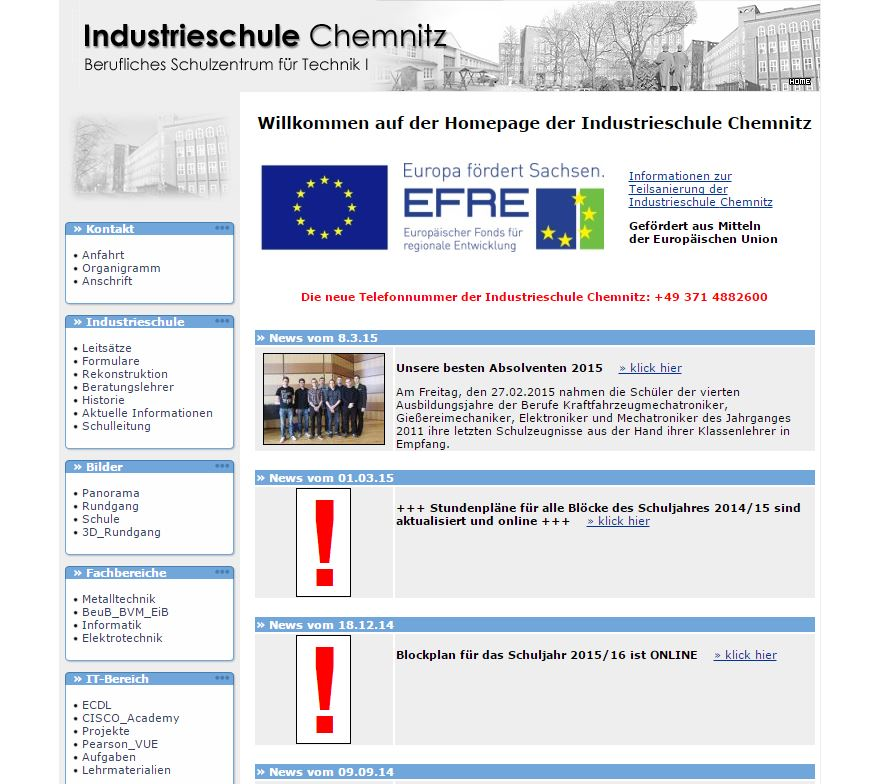
\includegraphics[width=0.80\textwidth]{./Bilder/oldpage.jpg}
	\caption{Main menue of the previous school homepage}
	\label{fig:pageOld}
\end{figure}
The main points of criticism where the missing ease of use; i.e. the old site was not responsive and barrier-free. Also 
the missing content management system complicated administration and updating the page. Furthermore the logical 
menu structure needed revision.

\subsection{Project Objective}
\label{sec:ProjectObjective}
The task of the new homepage is to provide information about the school, its offers and the school life. 
Furthermore it should be applicable to do public relations work, publish news and supply students, 
their parents and the companies of the trainees with materials. Last but not least the website reflects 
the schools media competence for the broad public.\\

It has been decided in advance that the website should be equipped with a stable updateable backend. 
The appearance of the new website was decided to be plain and functional according to the \textit{Modern UI} 
by Microsoft \cite{METRO} and fulfill today's requirements for comfort, be responsive and barrier-free. 
A further challenge is the visualisation of the timetables. The schools timetables are 
generated by an external program and need to be transformed into HTML.
\selectlanguage{ngerman}
\selectlanguage{ngerman}
% !TEX root = ../Projektdokumentation.tex
\section{Projektplanung} 
\label{sec:Projektplanung}

\subsection{Ressourcenplanung}
\label{sec:Ressourcenplanung}
Die Projektarbeit entstand sowohl in den Räumlichkeiten und PCs 
des Berufschulzentrums, sowie ihre privaten Rechner zuhause.
\subsubsection{Technische Ressourcen}
\label{sec:TechnischeRessourcen}
Als \acs{CMS} wurde TYPO3\footnote{\url{www.typo3.org}} eingesetzt, da hier auch eine komplexere 
Rechteverwaltung möglich ist und sich auch mehrsprachige Projekte
gut realisieren lassen. Zudem ist dieses System quelloffen und verfügt
über eine große aktive community.\\
Für die Verwaltung der Datenbank wird MySQL\footnote{\url{www.mysql.com}}


todo:mysql; sever(url; ip; apache)
\subsubsection{Personalplanung}
\label{sec:Personalplanung}
\subsection{Seitenstrucktur}
\label{sec:Seitenstrucktur}
\subsection{Designplanung}
\label{sec:Designplanung}
% !TEX root = ../Projektdokumentation.tex
\section{Projektvorbereitung} 
\label{sec:Projektvorbereitung}
\subsection{Projektumfeld}
\label{sec:Projektumfeld}
\subsection{Vorgaben}
\label{sec:Vorgaben}
\subsection{Zielgruppenanalyse}
\label{sec:Zielgruppenanalyse}
\subsection{Stand zu Begin der Projektphase}
\label{sec:StandZuBeginDerProjektphase}

\subsection{Seitenstruktur}
\label{sec:Seitenstruktur}
\begin{figure}[ht]
	\centering
	\includegraphics[width=0.80\textwidth]{./Bilder/Men�struktur}
	\caption{Grobe Men�struktur}
	\label{fig:menuStruct}
\end{figure}
In den vorausgehenden Besprechungen wurden diverse Strukturierungsstrategien eruiert. 
In Abb. \ref{fig:menuStruct} ist eine vereinfache Darstellung der geplanten
Men�strukturierung dargestellt.


\subsection{Designentwurf}
\label{sec:Designentwurf}
Beim Entwerfen des Designs sind mehrere Faktoren mit eingeflossen. Das Hauptaugenmerk
lag hierbei darauf, dass die �ffentliche Wahrnehmung der Medienkompetenz der Schule
stark von der Gestaltung der Internetpr�senz abh�ngt.
Au�erdem sollte mit einem modernen, schlichtem Design die \acs{CI} gest�rkt, sowie m�glichst 
viele Zielgruppen erreicht werden.\\
Zur Verbesserung der Corporate Identity lag also die erste Aufgabe in der Neugestaltung des 
Logos in Verbindung mit dem Banner. Hierbei musste, wie beim Rest der Seite vorallem darauf 
geachtet werden, die Schulfarben passend einflie�en zu lassen. Insgesamt wurde zur Verwaltung 
und Bereitstellung vieler Inhalte und Informationen ein sehr �bersichtliches Design ben�tigt.
Au�erdem musste zur Abbildung von Neuigkeiten eine passende Darstellungsform gefunden 
werden.\\
Die Herausforderung bestand darin, viele Informationen und Materialien �bersichtlich in einem
modernen und responsiven Design zu vereinen.
\todo{Grobentwurf Bild anf�gen}
\input
% !TEX root = ../Projektdokumentation.tex
\section{Umsetzung und Deployment} 
\label{sec:Umsetzung und Deployment}

\subsection{Skizzen und Screen-Design}
\label{sec:Skizzen und Screen-Design}
Jede Idee hat ihren Anfang auf einem Stück Papier. Wireframes sind unabdingbar, sie stellen die wichtigsten Funktionen einer 
Seite dar und dienen als Vorlage für das spätere Screen-Design. In Photoshop wurden daraufhin in mehreren Iterationen Screen-Designs
erstellt. Der finale Entwurf bildet dann die Basis für einen Prototyp.
\todo{Verweis auf Entwürfe?}

\subsection{Prototyping mit HTML und CSS}
\label{sec:Prototyping mit HTML und CSS}
Bevor das Design in TYPO3 integriert werden kann, ist es wichtig einen statischen Prototypen in HTML und CSS zu schreiben. 
In diesem Klickdummy können Fehler im Design rasch gefunden und entsprechende Lösungen entwickelt werden. Im Browser kann 
man zudem schnell improvisieren, sodass Probleme bei der User Experience - besonders im mobilen Bereich - oder der 
Barrierefreiheit schneller gelöst werden können als das in einem grafischen Entwurf der Fall ist. Sobald der Prototyp final ist,
kann damit begonnen werden, ihn mit dynamischen Inhalten zu befüllen.

\subsection{Lokale Umgebung einrichten}
\label{sec:Lokale Umgebung einrichten}
Damit keiner auf der Live-Umgebung direkt arbeitet, ist es notwendig eine geeignete Entwicklungsumgebung lokal zu errichten.
Darauf kann jeder Entwickler seine Arbeit unabhängig von anderen Entwicklern durchführen. Mit XAMPP wurde bei jedem eine lokale 
TYPO3-Installation aufgesetzt, auf der gearbeitet werden konnte. XAMMP richtet einen lokalen Apache-Server mit MySQL-Anbindung 
und einer aktuellen PHP-Version ein. Darauf kann dann eine TYPO3-Umgebung aufgesetzt werden.

\subsection{TYPO3 Integration}
\label{sec:TYPO3 Integration}
Eine nackte TYPO3-Installation und ein Prototyp allein bilden noch keine Webseite. Deswegen ist es notwendig, den erstellten 
Prototyp, der das Basistemplate der neue Website darstellt, mit dynamischen Inhalten zu befüllen. In TYPO3 wird dies durch 
TypoScript und der Template-Engine Fluid erreicht. Der Prototyp wird dabei in ein Fluid-Template überführt, in dem sogenannte 
Marker mit Inhalten ersetzt werden. Solche Inhalte sind z. B. Menüs, im Back-End angelegte Inhaltselemente, Header- und 
Footer-Bereiche der Seite.\\
Zur Integration gehört auch das Installieren von Extensions und die Einbindung deren Konfigurationsdateien. So wird 
beispielsweise die Extension realURL dazu benutzt, die URLs in ein für Menschen lesbares Format zu bringen.

\subsection{Entwicklung Stundenplan}
\label{sec:Entwicklung Stundenplan}
Die Schulstundenpl\"ane wurden bisher durch ein Programm erstellt, welches 
Dateien im txt-Format generiert. Diese \acs{ANSI}-kodierten Dateien enthalten, 
durch Tabulatoren getrennt, die Auflistung der R\"aume, F\"acher und Lehrer.
Da dieses Programm weiter durch den Auftraggeber genutzt werden soll, war 
es notwendig eine Konvertierung der Rohdaten in \acs{HTML} vorzunehmen.\\
Durch die M\"oglichkeit diese Dateien im Backend des \acs{CMS} hochzuladen, wurde eine 
Ordnerstruktur eingef\"uhrt, die diese Dateien nach Bl\"ocken trennt. 
Zus\"atzlich vereinfacht diese Struktur die Darstellung der Bl\"ocke und Klassen. Die Programmierung 
des Plugins zur Darstellung der Stundenpl\"ane begann mit dem Auslesen der Verzeichnisse, um einen 
\"uberblick \"uber alle verf\"ugbaren Dateien zu gewinnen und eine Auswahl f\"ur den Nutzer zur Verf\"ugung 
zu stellen. Nachdem der Nutzer den gew\"unschten Plan ausw\"ahlt, wird die entsprechende Datei 
ausgelesen, \acs{geparst}, in eine \acs{Array}struktur gebracht, um anschlie\ss{}end in Tabellenform angezeigt 
zu werden. Die Anzeige erfolgt \"uber Fluid, eine Extension von TYPO3 um die Gestaltung von Templates 
zu vereinfachen und um logische Operationen zu erweitern.

\subsection{Entwicklungen unter Versionskontrolle stellen}
\label{sec:Entwicklungen unter Versionskontrolle stellen}
Um eine einheitliche Versionierung und einen kontrollierten Entwicklungsprozess sicherstellen zu können, wurde die Extension
Stundenplan unter Versionskontrolle durch Git gestellt. Dadurch können parallele Arbeiten schnell und sicher zusammengeführt 
und bei Problemen die Änderungshistorie durchsucht und ggf. alte Stände zurückgeholt werden. Git stellt alle Dateien in einem 
Repository zusammen. Darunter befinden sich neben dem Quellcode zur Darstellung der Stundenpläne auch das Fluid-Template sowie 
alle Bilder, CSS-, und JavaScript-Dateien.\\
Entwickler können ihre Änderungen, die sie lokal gemacht haben, an diesen zentralen Ort senden und durch einen Merge werden 
die Änderungen mit der bisherigen Version zu einer neuen Version verschmolzen. Das Repository befindet ist derzeit unter Github 
(https://github.com/darthnorman/industrieschule-stundenplan), ist öffentlich zugänglich und kann von jedem heruntergeladen 
und geforkt werden.

\subsection{Deployment}
\label{sec:Deployment}
Neben Ersteinrichtung des Servers und Installation von ben\"otigten \acs{Extension}s wurde ein 
\acs{Datenbankdump} mittels phpMyAdmin eingespielt. Um die Stundenplan-\acs{Extension} einzubinden,
musste diese zun\"achst \acs{getaggt} werden, bevor sie im Anschluss aufgespielt wurde.

\todo{Testing?}

\subsection{Redakteuersdokumentation}
\label{sec:Redakteuersdokumentation}
Um den Redakteuren, welche die Seite weiter betreuen, die Arbeit mit dem \acs{CMS} zu erleichtern, 
wurde eine Redakteuersdokumentation angefertigt. Diese umfasst neben den grundlegenden Kenntnissen im Umgang mit TYPO3 
einen Leitfaden zur Handhabung des \acs{Back-End}s das Erstellen von Seiten und Inhalten wie Bilder, Texte, Neuigkeiten 
und Stundenpläne. Weiterhin wird die Rechte- und Rollenverteilung des Portals offen gelegt und auf sonstige Eigenheiten 
des Portals eingegangen.
\todo{Doku in den Anhang}
%% Table generated by Excel2LaTeX from sheet 'Dokumentation'
\begin{tabular}{llll}
\rowcolor{heading}\textbf{Vorgang} & \textbf{Geplant} & \textbf{Tatsächlich} & \textbf{Differenz} \\
1. Erstellen der Benutzerdokumentation & 2 h   & 2 h   &  \\
\rowcolor{odd}2. Erstellen der Projektdokumentation & 6 h   & 8 h   & +2 h \\
3. Programmdokumentation & 1 h   & 1 h   &  \\
\end{tabular}

\selectlanguage{english}
% !TEX root = ../Projektdokumentation.tex
\section{Conclusion} 
\label{sec:Conclusion}

\subsection{Acknowledgment}
The Authers like to thank Mr. Ciborra, Mr. Müller and Principal Hunger 
for the opportunity to work on this interesting and challenging project 
and for their support during its implementation.



% \begin{itemize}
	% \item Wurde das Projektziel erreicht und wenn nein, warum nicht?
	% \item Ist der Auftraggeber mit dem Projektergebnis zufrieden und wenn nein, warum nicht?
	% \item Wurde die Projektplanung (Zeit, Kosten, Personal, Sachmittel) eingehalten oder haben sich Abweichungen ergeben und wenn ja, warum?
	% \item Hinweis: Die Projektplanung muss nicht strikt eingehalten werden. Vielmehr sind Abweichungen sogar als normal anzusehen. Sie müssen nur vernünftig begründet werden (\zB durch Änderungen an den Anforderungen, unter-/überschätzter Aufwand).
% \end{itemize}

% \paragraph{Beispiel (verkürzt)}
% Wie in Tabelle~\ref{tab:Vergleich} zu erkennen ist, konnte die Zeitplanung bis auf wenige Ausnahmen eingehalten werden.
% \tabelle{Soll-/Ist-Vergleich}{tab:Vergleich}{Zeitnachher.tex}



% \begin{itemize}
	% \item Was hat der Prüfling bei der Durchführung des Projekts gelernt (\zB Zeitplanung, Vorteile der eingesetzten Frameworks, Änderungen der Anforderungen)?
% \end{itemize}


% \subsection{Outlook}
% \label{sec:Outlook}

% \begin{itemize}
	% \item Wie wird sich das Projekt in Zukunft weiterentwickeln (\zB geplante Erweiterungen)?
% \end{itemize}

\selectlanguage{ngerman}

% Literatur ------------------------------------------------------------------
\clearpage
\renewcommand{\refname}{Quellenverzeichnis}
\bibliography{Bibliographie}
\bibliographystyle{Allgemein/natdin} % DIN-Stil des Literaturverzeichnisses
% !TEX root = Projektdokumentation.tex
\clearpage
\addsec{Eidesstattliche Erklärung}

Wir, \autorName, versichern hiermit, dass wir unsere \textbf{\betreff} mit dem
Thema
\begin{quote}
\textit{\kompletterTitel}
\end{quote}
selbständig verfasst und keine anderen als die angegebenen Quellen und Hilfsmittel benutzt haben,
wobei wir alle wörtlichen und sinngemäßen Zitate als solche gekennzeichnet haben. Die Arbeit
wurde bisher keiner anderen Prüfungsbehörde vorgelegt und auch nicht veröffentlicht.\\[6ex]

\abgabeOrt, den \abgabeTermin


\rule[-0.2cm]{5.5cm}{0.5pt}

\textsc{\autorName}


% Anhang ---------------------------------------------------------------------
%\clearpage
%\appendix
%\pagenumbering{roman}
%input{Anhang}

\end{document}
